%!TEX root = ../DSGEnotes.tex
\section{傅里叶分析}
\label{sec:fourier-analysis}

我们可以这样理解分析(analysis):将研究对象分解成小块来分别研究。那么我们可以这样理解傅里叶分析(Fourier analysis):将研究对象(方程)分解为小块,即不同的弦波(sinosoids),每个小快都以有限的速度变化。例如这个方程
\begin{equation*}
  f(t) = 3 \cos 2 \pi t + 19 \sin 4\pi t - 0.14 \cos 7 \pi t,
\end{equation*}
可以分解为
\begin{equation*}
  \begin{split}
    f(t) & = 3 A + 19 B - 0.14 C,
  \end{split}
\end{equation*}
其中$A,B,C$分别表示角频率(angular frequency)\index{angular frequency \dotfill 角频率}为$2 \pi, 4 \pi, 7 \pi$的弦波。

但对于这样的方程
\begin{equation*}
\begin{split}
    f(t) &  = \exp \left( - \alpha \left| t \right| \right), \\
    f(t) & = \begin{cases}
    1, & \left| t \right| < 1 \\
    2, & \left| t \right| > 1
    \end{cases},
\end{split}
\end{equation*}
甚至更复杂一些的方程,该如何做傅里叶分析?

在开始正式介绍之前,有必要做一些简单的概念界定,见表\ref{tab:fourier-analysis-definition}。

\begin{table}[htbp]
\caption{傅里叶分析的常见概念界定}
%\begin{flushleft}
\begin{tabular}{|l|c|c|}
\hline
 & 连续方程 $f(t)$ & 离散方程 $f_{n} \equiv f \left( n \Delta t \right), n \in \mathcal{Z}$\\ \hline
无限域 $- \infty < t < \infty$  & 傅里叶变换 (Fourier transform) \index{Fourier transform! \dotfill 傅里叶变换}& 半离散傅里叶变换 (Semidiscrete Fourier transform)\index{Fourier transform!Semidiscrete \dotfill 半离散傅里叶变换} \\ \hline
有限域 $- \frac{T}{2} < t < \frac{T}{2}$ & 傅里叶级数 (Fourier seires)\index{Fourier series \dotfill 傅里叶级数} & 离散傅里叶变换 (Discrete Fourier transform)\index{Fourier transform!Discrete \dotfill 离散傅里叶变换} \\ \hline
\end{tabular}
%\end{flushleft}
\label{tab:fourier-analysis-definition}
\end{table}

\subsection{傅里叶变换}
\label{sec:fourier-transform}
我们先从表\ref{tab:fourier-analysis-definition}左上角的傅里叶变换开始介绍,即连续方程$f(t)$在无限时间区间$(-\infty, \infty)$的求积问题。
\begin{equation}
  \label{sec:fourier-transform-definition}
  \tilde{f} \left( \omega \right) =
  \frac{1}{2 \pi} \int_{-\infty}^{\infty}
  \exp \left( - i \omega t \right) f(t) \, \mathrm{d} t,
\end{equation}
其中$f \left( \omega \right)$是一个关于频率$\omega$的方程,方程形式反映了在频率域$\omega$中表现出的非线性(指数)强烈程度。

现在基于傅里叶变换式\eqref{sec:fourier-transform-definition}来回顾前面的问题:如何将方程$E_{\alpha}(t) = \exp \left( - \alpha \left| t \right| \right)$分解为一组弦波组合的形式?其基本思路是,通过将所有关于频率$\omega$的弦波曲线加总来重写原方程$\exp \left( - \alpha \left| t \right| \right)$,某一弦波的频率越大,振幅(amplitude)。
\begin{equation*}
  \begin{split}
    \widetilde{E}_{\alpha} \left( \omega \right)
    & = \frac{1}{2 \pi}
    \int_{-\infty}^{\infty} \exp \left( - i \omega t \right) \exp \left( - \alpha \left| t \right| \right) \, \mathrm{d} t \\
    & = \frac{1}{2 \pi} \left\{
    \int_{-\infty}^{0} \exp \left[ \left( - i \omega + \alpha \right) t \right] \, \mathrm{d} t
    + \int_{0}^{\infty} \exp \left[ \left( - i \omega - \alpha \right) t \right]
    \right\} \\
    & = \frac{1}{2 \pi}
    \left[
    \frac{1}{\alpha - i \omega}
    - \frac{1}{\alpha + i \omega}
    \right] \\
    & = \frac{\alpha}{\pi \left( \alpha^{2} + \omega^{2} \right)},
  \end{split}
\end{equation*}
注意,这里所说的``频率"$\omega$越大或越小,是相对于参数$\alpha$而言的:$\alpha$越大,指数方程$E_{\alpha}(t)$越快衰减至$0$,我们就越需要增加$\widetilde{E}_{\alpha}(\omega)$的振幅,利用更高振幅的弦波来近似原方程。下面将作进一步说明。

\subsubsection{一些概念}
\begin{equation*}
  y = A \sin \left( B x + c \right) + D,
\end{equation*}
其中
\begin{itemize}
  \item $A$表示振幅,
  \item $\frac{B}{2 \pi}$表示周期,$\text{频率} = \frac{1}{\text{周期}}$,
  \item $- \frac{C}{B}$表示相位的(水平)移动,
  \item $D$表示相位的(垂直)移动。
\end{itemize}

\begin{figure}[htbp]
   \caption{傅里叶变换}
  \centering
  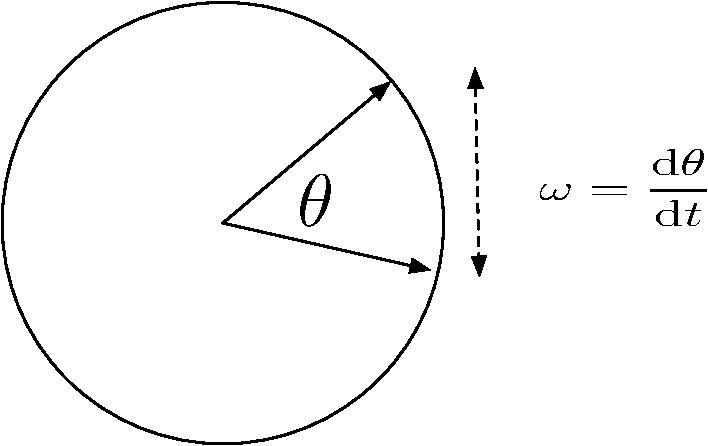
\includegraphics[width=8cm]{./Figures/20180302-frequencies-etc.pdf}
  \label{fig:fourier-basic-concepts}
%
%  \small{Source: PBOC.}
\end{figure}
图\ref{fig:fourier-basic-concepts}中
\begin{itemize}
  \item $\omega = \frac{2 \pi}{T} = 2 \pi \nu = %\frac{\nu}{r}
  = \frac{\mathrm{d} s}{\mathrm{d} t} \cdot \frac{1}{r} = \frac{\mathrm{d} \theta}{\mathrm{d} t}$
  \item $\omega$,角频率(angular frequency)\index{angular frequency \dotfill 角频率},是对物体旋转速度快慢的度量,单位如弧度/秒(radian/second)。
  \item $T$,周期,单位如秒。
  \item $\nu$,线频率(linear frequncy),单位如赫兹(Hertz),$1 Hertz = 1\text{次/秒}$。
  %\item 绕轴旋转的线速度,单位如米/秒。
  \item 旋转的半径,单位如米。
\end{itemize}

\subsubsection{线频率和角频率}
\label{sec:fourier-frequency-linear-angular}
对于一个给定的弦波方程如$\sin \omega t$或$\exp \left[ - i \omega t\right]$等,严格说来我们需要将其中的频率$\omega$理解为角频率$\omega$(angular frequency)\index{angular frequency \dotfill 角频率},表示相角旋转速度的快慢,单位如角每秒(radian per second)。线频率(linear frequency)可写为\index{linear frequency \dotfill 线频率}$\nu = \frac{\omega}{2 \pi}$,表示这一过程自我重复的频率,单位如赫兹。例如,一个钟摆4秒钟转一圈,那么
\begin{itemize}
  \item 周期$T=4$,
  \item 角频率$\omega = \frac{2 \pi}{T} = \frac{\pi}{2} \approx 1.57 Rad/s$,
  \item 线频率$\nu = \frac{1}{T} = 0.25 Hz$。
\end{itemize}

\subsubsection{域}
\label{sec:fourier-domains}

\eqref{sec:fourier-transform-definition}对原方程$f(t)$作傅里叶变换,生成近似方程$\tilde{f}(\omega)$,二者等价但处于不同的域中。$f(t)$的解释变量是(时间)$t$,$\tilde{f}(\omega)$的解释变量是频率$\omega$,从这个角度可以说,$f(t)$是在时间域中,$\tilde{f}(\omega)$是在频率域中。

福利也分析也可用于原方程$f$的解释变量不是时间的情况,例如可以是方位$x$,对应的傅里叶变换处于空间频率$k$中,有时也称波数(wavenumber)\index{wavenumber \dotfill 波数}。更多例子见下表。

\begin{table}[htbp]
\caption{原方程域和傅里叶变换方程域}
%\begin{flushleft}
\begin{tabular}{|l|cccc|}
\hline
& 原变量 & 原域 & 傅里叶变量& 傅里叶域 \\ \hline
信号处理 & 时间$t$ & 时间域 & 频率$\omega$ & 频率域 \\
光学 & 方位$x$ & 实空间 & 波数$k$ & $k$空间 \\
量子力学 & 方位$x$ & 方位空间 & 动量(momentum)$p$ & 动量空间 \\
固体物理学 & 点阵向量$L$ & 实空间 & 布洛赫向量(Bloch vector) $k$ & 晶体动量空间(crystal momentum space)
\\ \hline
\end{tabular}
%\end{flushleft}
\label{tab:fourier-domain-definition}
\end{table}

\subsubsection{单位}
实际研究过程中需要牢记$f(t)$和$\tilde{f}(\omega)$的单位不同。以\eqref{sec:fourier-transform-definition}为例,RHS中有$\mathrm{d} t$,LHS中没有。因此
\begin{equation*}
    \tilde{f}\text{的单位} = f\text{的单位} \times \text{时间} = \frac{f\text{的单位}}{\text{频率}},
\end{equation*}
如果$f$的单位是伏特(Volt),那么$\tilde{f}$的单位是伏特秒,或者伏特每赫兹。

\subsubsection{傅里叶变换的性质}
\label{sec:fourier-properties}
由定义\eqref{sec:fourier-transform-definition}可得,傅里叶变换具有如下性质,我们将分别作说明。
\begin{itemize}
  \item 导数的傅里叶变换
  \item 傅里叶变换的导数
  \item 实值方程的傅里叶变换
\end{itemize}

\textit{导数的傅里叶变换}。对于某一给定方程$f(x)$,如果我们可以求得其傅里叶变换$\tilde{f}(k)$,那么$f(x)$的导数也很容易写出。首先写出$f(t)$的傅里叶综合表达式(Fourier synthesis equation, 第\ref{eq:fourier-series-synthesis}节)
\begin{equation*}
  f(x) = \int_{-\infty}^{\infty} \tilde{f}(k) \exp \left( i k x \right) \, \mathrm{d} k,
\end{equation*}
两侧同时对$x$求导
\begin{equation*}
  \frac{\mathrm{d}}{\mathrm{d} x}f(x)
  = \int_{-\infty}^{\infty} i k \tilde{f}(k) \exp \left( i k x \right) \, \mathrm{d} k,
\end{equation*}
上式的RHS是对$\left( i k \widetilde{f} (k) \right)$的逆傅里叶变换(Definition \ref{definition:fourier-transformation});因此可以将RHS看作是$\frac{\mathrm{d}}{\mathrm{d} x}f(x)$的傅里叶变换,即
\begin{equation}
  \label{eq:fourier-derivative-ft-eq}
  \mathcal{F}\left[ f(x) \right]
  = \tilde{f}(k) \Rightarrow \mathcal{F}
  \left[
  \frac{\mathrm{d}}{\mathrm{d} x}f \left( x \right)
  \right] = i k \tilde{f}(k).
\end{equation}

也可以重复上述过程求解高阶导数,如
\begin{equation}
  \label{eq:fourier-derivative-ft-eq-higher}
  \mathcal{F} \left[ f(x) \right] = \tilde{f}(k)
  \Rightarrow
  \mathcal{F} \left[ \frac{\mathrm{d}}{\mathrm{d} x} f(x) \right]
  = i k \tilde{f} (k)
  \Rightarrow
  \mathcal{F}
  \left[
  \frac{\mathrm{d}^{2}f}{\mathrm{d} x^2} \right]
  = - k^{2} \tilde{f}(k).
\end{equation}

\textit{傅里叶变换的导数}。
类似地,对傅里叶变换\eqref{sec:fourier-transform-definition}
\begin{equation*}
  \tilde{f} \left( k \right) =
  \frac{1}{2 \pi} \int_{-\infty}^{\infty}
  \exp \left( - i k x \right) f(x) \, \mathrm{d} x
\end{equation*}
两侧求$k$的导数有
\begin{equation*}
  \frac{\mathrm{d}}{\mathrm{d} k} \tilde{f}(k)
  = \int_{-\infty}^{\infty} - i x f(x) \exp \left( - i k x \right) \, \mathrm{d} x,
\end{equation*}
可见$\frac{\mathrm{d}}{\mathrm{d} k} \tilde{f}(k)$可以看成是方程$x \cdot f(x)$的傅里叶变换。因此有
\begin{equation}
  \label{eq:fourier-ft-derivative-eq}
  \mathcal{F}\left[ f(x) \right] = \tilde{f}(k)
  \Rightarrow \mathcal{F} \left[ x f(x) \right]
  = i \frac{\mathrm{d}}{\mathrm{d} k }\tilde{f}(k).
\end{equation}

不难看出,\eqref{eq:fourier-derivative-ft-eq} 和\eqref{eq:fourier-ft-derivative-eq}等价。

\textit{实值方程的傅里叶变换}。
如果$f(x)$是一个实值方程,那么它对应的傅里叶变换$\tilde{f}(k)$中所含有的信息中,相对于$k<0$的部分就是冗余信息:$\tilde{f}\left(k \right) \big|_{k <0 }$的信息可由$\tilde{f}\left(k \right) \big|_{k > 0}$的部分而获得。以定义式为例,对于$k<0$的情况下有
\begin{equation*}
\tilde{f}\left( - k \right) = \frac{1}{2 \pi} \int_{- \infty}^{\infty} f(x) \exp \left( i k x \right) \, \mathrm{d} x,
\end{equation*}
由于假定$f(x)$是一个实值方程,进一步可得
\begin{equation*}
%  \label{eq:fourier-real-valued-func}
  \tilde{f}(-k) =
  \left[
  \frac{1}{2 \pi} \int_{- \infty}^{\infty} f(x) \exp \left( - i k x \right) \, \mathrm{d} x
  \right]^{*}
  = \tilde{f}^{*} (k).
\end{equation*}


\subsection{脉冲方程的傅里叶变换}
\label{sec:fourier-function-types}
介绍几种常见的傅里叶变换。

\subsubsection{洛伦兹变换}
\label{sec:fourier-lorentzian-transformation}
以前文提到的方程为例
\begin{equation}
  \label{eq:fourier-lorentzian}
  E_{\alpha} \left( x \right) = \exp \left( - \alpha \left| x \right| \right), \quad \widetilde{E}_{\alpha} \left( k
  \right) = \frac{
  \alpha
  }{
  \pi \left( \alpha^{2} + k^{2} \right)
  }.
\end{equation}

$E_{\alpha} \left( x \right)$和$\widetilde{E}_{\alpha} \left( k
\right)$都可以被看作是某种脉冲方程(pulse functions):它们都在初始点$x_{0} ,k_{0}$处附近有最大值,又随着$x \rightarrow \infty$或$k \rightarrow \infty$而逐渐降低直至$0$,称为洛伦兹变换(Lorentzian function)\index{Lorentzian function \dotfill 洛伦兹方程}。两个方程的宽度均与参数$\alpha$有关,但影响方向相反:$\alpha$的值越大,实空间中的脉冲越弱、宽度越窄,傅里叶空间中的脉冲越强、宽度越宽,如图\ref{fig:fourier-lorentzian-trans}所示。
\begin{figure}[htbp]
   \caption{洛伦兹方程$(\alpha = 2)$}
  \centering
  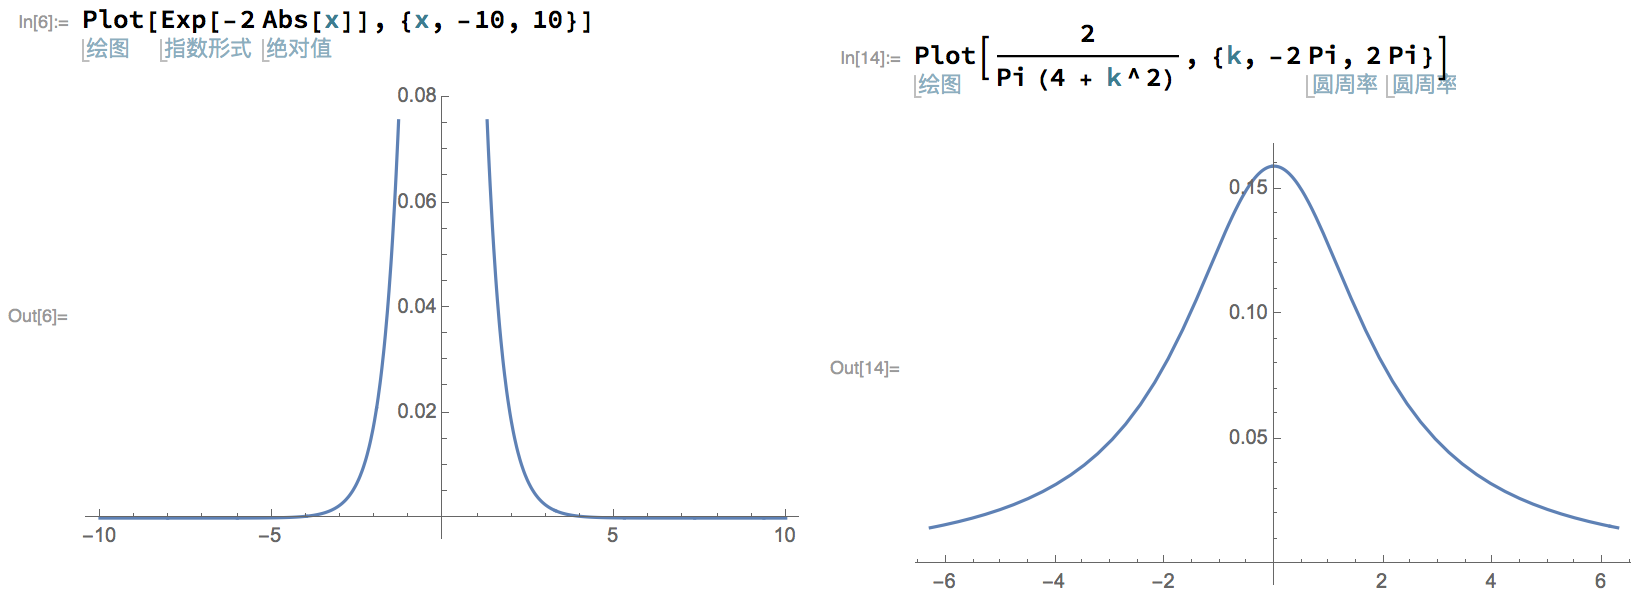
\includegraphics[width=14cm]{./Figures/20180304-lorentzian-example.png}
  \label{fig:fourier-lorentzian-trans}
%
%  \small{Source: PBOC.}
\end{figure}

我们将脉冲的一个半峰全宽(full width at half maximum, FWHM)\index{full width at half maximum(FWHM) \dotfill 半峰全宽}定定义为,在方程的一个周期中,前后两个方程值等于一个峰值一半的点之间的距离。根据这个定义,$E_{\alpha}(x)$的峰值为$1(x=0)$,并且在$x \pm (\ln 2) / \alpha$时,值为峰值的一半,因此有
\begin{equation}
  \label{eq:fourier-lorentzian-fwhm-e}
  FWHM \left[ E_{\alpha} (x) \right] = \frac{2 \ln 2}{\alpha},
  \end{equation}
$\widetilde{E}_{\alpha}(k)$的峰值为$\frac{1}{\pi \alpha} (k = 0)$,在$k = \pm \alpha$时,值为峰值的一半,
\begin{equation}
    \label{eq:fourier-lorentzian-fwhm-tilde-e}
    FWHM \left[ \widetilde{E}_{\alpha}(k) \right] = 2 \alpha.
\end{equation}

\eqref{eq:fourier-lorentzian-fwhm-e}和\eqref{eq:fourier-lorentzian-fwhm-tilde-e}联立有
\begin{equation}
  \label{eq:fourier-lorentzian-fwhm-product}
  FWHM \left[ E_{\alpha} (x) \right] \cdot FWHM \left[ \widetilde{E}_{\alpha}(k) \right] = 4 \ln 2,
\end{equation}
注意:单个原方程及洛伦兹变换方程的FWHM与$\alpha$有关;两个$FWHM$的乘积则与$\alpha$无关:所有洛伦兹脉冲方程族$\left\{ E_{\alpha}(t) \right\}$都具有这样的特征。

\subsubsection{高斯变换}
\label{sec:fourier-gaussian}
设一个宽度为$\sigma$的高斯方程(Gaussian function)\index{Gaussian function \dotfill 高斯方程}\footnote{高斯方程族中有不同的类型,简要介绍见第\ref{sec:fourier-tips-gaussian}节。}
\begin{equation*}
  G_{\sigma}(x) = \exp \left( - \frac{x^{2}}{\sigma^{2}}\right),
\end{equation*}
那么其傅里叶变换
\begin{equation*}
  \begin{split}
    \widetilde{G}_{\sigma} \left( k \right)
    & = \frac{1}{2 \pi}
    \int_{-\infty}^{\infty} \exp \left( - i k x \right)
    G_{\sigma} \left( x \right) \, \mathrm{d} x \\
    & = \frac{1}{2 \pi}
    \int_{-\infty}^{\infty}
    \underbrace{
    \exp
    \left(
    - i k x - \frac{x^{2}}{\sigma^{2}}
    \right)
    }_{\eqqcolon \mathcal{A} }
    \, \mathrm{d} x,
  \end{split}
\end{equation*}
RHS的被积方程
\begin{equation*}
  \begin{split}
    \mathcal{A} & = \frac{1}{\sigma^{2}}
    \left( x^{2} + i k x \sigma^{2} \right) \\
    & = \frac{1}{\sigma^{2}}
    \left(
    x + \frac{1}{2} i k \sigma^{2}
    \right)^{2} + \frac{1}{4} k^{2} \sigma^{2} \\
    & = \frac{1}{2 \pi} \exp \left( - \frac{1}{4} k^{2} \sigma^{2} \right)
    \underbrace{
    \int_{-\infty}^{\infty} \exp
    \left[
    - \frac{1}{\sigma^{2}}
    \left( x + \frac{1}{2} i k \sigma^{2} \right)^{2}
    \right] \, \mathrm{d} x
    }_{= \sigma \cdot \sqrt{\pi}} \\
    & = \frac{\sigma}{2 \sqrt{\pi}} \exp \left( - \frac{1} {4} k^{2} \sigma^{2} \right),
  \end{split}
\end{equation*}

可见$\widetilde{G}_{\sigma}(k)$也是一个$k$空间中的高斯方程,其宽度与原方程$G_{\sigma}(x)$的宽度成等比例
\begin{equation*}
  \widetilde{G}_{\sigma} \propto \exp \left( - \frac{k^{2}}{\tilde{\sigma}^{2}} \right) = G_{\tilde{\sigma}} \left( k \right), \quad \tilde{\sigma} \equiv \frac{2}{\sigma}.
\end{equation*}

此外
\begin{equation}
    \label{eq:fourier-gaussian-fwhm-product}
  \begin{split}
    FWHM \left[ G_{\sigma} \left( x \right) \right]
    & = 2 \sqrt{ \ln 2} \sigma, \\
    FWHM \left[ G_{\sigma} \left( x \right) \right] \cdot FWHM \left[ \widetilde{G}_{\sigma} \left( x \right) \right]
    & = \left( 2 \sqrt{\ln 2} \sigma \right) \cdot
    \left( \frac{4 \sqrt{\ln 2}}{\sigma}\right) = 8 \left( \ln 2\right)^{2},
  \end{split}
\end{equation}
可见单个原高斯方程及高斯变换方程的FWHM与$\alpha$有关;两个$FWHM$的乘积则与$\alpha$无关:所有高斯脉冲方程族$\left\{ G_{\sigma}(x) \right\}$都具有这样的特征。

\subsection{非脉冲方程的傅里叶变换}
\label{sec:fourier-non-pulse-functions}
洛伦兹变换和高斯变换都属于脉冲方程,特点是初始点附近有峰值,随着$x$($k$)逐渐增大而慢慢回落至$0$。如何求得非脉冲方程的傅里叶变换,如$f(x) = 1, \, f(x)=x, $或$f(x) = x^{2}$呢?

一种求解思路是,考虑\eqref{eq:fourier-lorentzian}在$\lim_{\alpha \rightarrow 0}$时的情况,实值方程趋近于$1$
\begin{equation*}
  \lim_{\alpha \rightarrow 0} E_{\alpha}(x) \rightarrow 1.
\end{equation*}

而它的洛伦兹变换$\widetilde{E}_{\alpha}(k)$的求解则较为复杂,第一它的宽度变窄了$FWHM \widetilde{E}_{\alpha} = 2 \alpha$;第二它的高度变高了$\widetilde{E}_{\alpha} \left( 0 \right) = \frac{1}{\pi \alpha}$。随着$\alpha \rightarrow 0$的极限情况出现,$\lim_{\alpha \rightarrow 0} \widetilde{E}_{\alpha}(k)$变得极窄、极高,就成为狄拉克方程(Delta Dirac function, 第\ref{sec:kernel-gaussian-dirac}节) \index{Delta Dirac function \dotfill 狄拉克方程}
\begin{equation}
  \label{eq:fourier-non-pulse-dirac}
  \lim_{\alpha \rightarrow 0} \widetilde{E}_{\alpha}(k) = \lim_{\alpha \rightarrow 0} \frac{
  \alpha
  }{\pi \left( \alpha^{2} + k^{2} \right)}
  \equiv \delta (k) = \begin{cases}
  + \infty & k = 0, \\
  0 & k \neq 0,
\end{cases} \quad \Rightarrow \int_{- \infty}^{\infty} \delta (k) \, \mathrm{d} k = 1.
\end{equation}

对应地,非脉冲方程$f(x) =1$的傅里叶变换可以写作
\begin{equation}
  \label{eq:fourier-non-pulse-ftran-1}
  f(x) \equiv 1 \Rightarrow \tilde{f}(k) = \delta(k),
\end{equation}
可以这么理解:$f(x) \equiv 1$是一个频率为$0$的弦波。对$f(x)$做傅里叶转换,分解为若干弦波之和,在这一系列弦波中,我们将除了第一条(对应频率为$0$)之外的其他全部弦波曲线的系数值均设为$0$。

在此基础上,利用\eqref{eq:fourier-non-pulse-ftran-1}和\eqref{eq:fourier-ft-derivative-eq},进一步可得到另外两个非脉冲方程的傅里叶变换
\begin{align}
  \label{eq:fourier-non-pulse-ftran-x1}
  f(x) = x \quad \Rightarrow \tilde{f}(k) = i \delta^{'}(k), \\
  \label{eq:fourier-non-pulse-ftran-x2}
  f(x) = x^{2} \quad \Rightarrow \tilde{f}(k) = - \delta^{''}(k),
\end{align}

其中$\delta'(k)$是狄拉克方程的导数,基于\eqref{eq:fourier-non-pulse-dirac}用分部积分法有
\begin{equation*}
  \int f(u) \delta^{'}(u) \mathrm{d} u =
  - \int f^{'}(u) \delta(u) \, \mathrm{d} u = - f^{'}(u),
\end{equation*}
可见$\delta'$可以被看做是和$\delta$相近的方程,二者只有一点不同:利用分部求积计算$\delta'$时产生了$- f'(0)$的变化,而$\delta$只产生$-f$的变化。

需要指出的是,对非脉冲方程的傅里叶变换如\eqref{eq:fourier-non-pulse-ftran-1}、\eqref{eq:fourier-non-pulse-ftran-x1}、\eqref{eq:fourier-non-pulse-ftran-x2},都不算是``好''的方程——它们甚至不是方程,而只是分布(比如狄拉克方程单独出现往往没有实际意义,它更多是与其他定义良好的方程配对出现在积分式中):这么说是因为$f(x)= \left\{ 1, x, x^{2} \right\} \notin L^{1}$,即它们不满足$\int_{-\infty}^{\infty} \left| f(x) \right| \, \mathrm{d}x < \infty$。
\footnote{$L^{1}$表示勒贝格空间,见第\eqref{sec:lesbegue-space}节。}
因此,\eqref{eq:fourier-non-pulse-ftran-x2}等傅里叶变换,往往更适合以算子的形式出现。

\subsection{原方程的平滑和傅里叶变换方程的衰减}
\label{sec:fourier-smoothness-decay}
通过前面的分析不难总结出一个一般规律:原方程$f(t)$越是(口语意义上的)不``平滑'',即随着解释变量$t$的变动而剧烈变动,其傅里叶变换$\tilde{f} \left( \omega \right)$随着$\omega$的衰减(decay)速度就越慢。反之亦然:$f(t)$越平滑,$\tilde{f} \left( \omega \right)$的衰减就越快。可以将$f(t)$的平滑特性表现为$f$的连续性和导数:
\begin{theorem}[佩利——维纳诸定理]
  \label{theorem:paley-wiener-theorems}
  如果$f(t)$和它的前$p-1$个导数都是连续的,但第$p$个导数是不连续的,并且变差有界(bounded variation),那么$\tilde{f}(\omega)$的衰减速度不低于$\left| \omega \right|^{- \left( p + 1 \right)} \big|_{\omega \rightarrow \infty}$。  这称为佩利——维纳诸定理(Paley-Wiener theorems)\index{Paley-Wiener theorems \dotfill 佩利——维纳诸定理}。
\end{theorem}
\begin{proof}
  一种证明方式见第\pageref{eq:ninc-cc-trape-fsynthesis-coef-boyd}页脚注。更详实的证明可参考如\cite[Sec. VI.4]{Yosida:1978ul},\cite[Theorem 4.1.2]{Agranovich:2015cv}。
\end{proof}

  尤其是,若$f(t) \in C^{\infty}$,\footnote{空间$C^{\infty}$中的方程连续,所有导数也都连续,可参考第\ref{sec:spaces-c}节。}那么在$\omega$值较大时,$\tilde{f}(\omega)$的衰减速度比任何多项式都快。这样的方程包括诸如$\exp \left( - \omega \right)$,$\exp \left( - \sqrt{\omega} \right)$,$\exp \left( - \omega^{2} \right)$等。

举例如洛伦兹方程$\exp \left( - \alpha \left| t \right| \right)$连续,但其一阶导数不连续,表现为在$t=0$处有跳跃,如图\ref{fig:fourier-lorentzian-trans}左侧。因此$p=1$。对应地,我们会看到它的傅里叶变换以等比于$\omega^{-2}$的速度衰减(当$\omega$的值较大时)。

再比如,方程$\exp \left( - \frac{t^{2}}{\sigma^{2}} \right) \in C^{\infty}$,那么其傅里叶变换$\widetilde{F} = \exp \left( - \frac{1}{4} \sigma^{2} \omega^{2} \right)$的衰减速度快于任意多项式。

\subsection{傅里叶级数}
\label{sec:fourier-seires}
现在来看表\ref{tab:fourier-analysis-definition}左下一栏,对应有限空间中连续方程$f(t)$的傅里叶分析,称为傅里叶级数。

假设$f(t)$是个关于$T$的周期方程(periodic function)\index{periodic function \dotfill 周期方程},即每隔$T$单位时间(秒,分,小时,天等)就自我重复一遍:
\begin{equation*}
  f(t+T) \equiv f(t), \quad \forall t.
\end{equation*}

假定$f(t)$符合傅里叶分析的条件,对应傅里叶变换
\begin{equation}
  \label{eq:fourier-series-def}
  \tilde{f}(\omega) = \frac{1}{2 \pi} \int_{-\infty}^{\infty}
  \exp \left( - i \omega t \right) f(t) \, \mathrm{d} \omega,
\end{equation}
随着角频率$\omega$和基准频率(base frequency) $
\omega_{0}=\frac{2 \pi}{T}$的关系不同,需要分两种情况来分析:
\begin{enumerate}
  \item $\omega$是$\omega_{0}$的整数倍。

  那么\eqref{eq:fourier-series-def}中的被积方程周期为$T$,每个宽度为$T$的子区间对总积分的作用相同,并且由于这样的子区间有无数个,我们有$\tilde{f} \left( \omega \right) = \infty$。
  \item $\omega$是$\omega_{0}$的整数倍。

  那么\eqref{eq:fourier-series-def}中的被积方程不是一个周期方程。我们可以将$f(t)$理解为两部分:一部分是$f(t)$,这是一个关于$T$的周期方程,另一部分是$\exp \left( - i \omega t \right)$,它只有在某些特定的时期才是周期方程,这些特定的时期是指不等于$T$的整数倍的时期。两部分的乘积导致被积方程不是一个周期方程。

  每个宽度为$T$的子区间都给总积分值产生同等程度的影响,但影响的大小(phase,相)是随机的。各个随机相的影响加总后相互抵消,$\tilde{f}(\omega) =0$。
\end{enumerate}

将上述两种情况汇总可见,在$f(t)$是一个周期方程的前提下
\begin{equation*}
  \tilde{f}(\omega) =
  \begin{cases}
    \infty, & \omega\text{是}\omega_{0}\text{的整数倍},\\
    0, & \text{否则}.
  \end{cases}
\end{equation*}

我们可以用三种数学形式将上式表达出来:
\begin{enumerate}
  \item 利用狄拉克方程,可将$T$-周期方程的傅里叶变换表示为
  \begin{equation}
    \label{eq:fourier-series-dirac}
    \tilde{f}(\omega) = \sum_{\nu = - \infty}^{\infty}
    \tilde{f}_{\nu} \cdot \delta \left( \omega - \nu \omega_{0} \right), \quad \omega_{0} \equiv \frac{2 \pi}{T}, \, \nu \in \mathcal{Z}.
  \end{equation}
  \item 对$T$-周期方程$f(t)$的傅里叶分解,只包括那些频率为$\omega_{\nu}$的弦波曲线,满足$\omega_{\nu} = \nu \cdot \omega_{0} = \frac{2 \nu \pi}{T}, \, \nu \in \mathcal{Z}$,记作
  \begin{equation}
    \label{eq:fourier-series-exponential}
    f(t) = \sum_{\nu \in \mathcal{Z}} \tilde{f}_{\nu} \cdot \exp \left( i \nu \omega_{0} t \right), \quad \omega_{0} = \frac{2 \nu \pi}{T}, \, \nu \in \mathcal{Z},
  \end{equation}
  我们又将\eqref{eq:fourier-series-exponential}称为傅里叶级数(Fourier series)\index{Fourier series \dotfill 傅里叶}的表达形式之一:复杂指数表达形式。

  \item 除此之外,也可以将傅里叶级数表达为另一种形式,即一组正弦函数和一组余弦函数之和
  \begin{equation}
    \label{eq:fourier-series-sin}
    f(t) = \sum_{\nu = 0}^{\infty} \tilde{a}_{\nu} \cdot \cos \left( \nu \omega_{0} t \right)
    + \sum_{\nu = 1}^{\infty} \tilde{b}_{\nu} \cdot \sin \left( \nu \omega_{0} t \right), \quad \nu \in \mathcal{Z}^{+}.
  \end{equation}
\end{enumerate}

\subsubsection{两种表达形式的比较}
  \eqref{eq:fourier-series-sin}中的$\nu$需要取正整数;\eqref{eq:fourier-series-exponential}则正负均可。除此而外,指数形式\eqref{eq:fourier-series-exponential}和弦波形式\eqref{eq:fourier-series-sin}等价,可以被看作是同一个$T$-周期方程$f(t)$的傅里叶级数分解。

来看两组系数$\left\{ \tilde{a}_{\nu}, \tilde{b}_{\nu} \right\}_{\nu \in \mathcal{Z}^{+}}$和$\left\{ \tilde{f}_{\nu} \right\}_{\nu \in \mathcal{Z}}$之间的关系。已知复杂指数$\exp \left( i \nu \omega_{0} t \right)$可表示为关于正弦和余弦函数的方程
\begin{equation}
  \label{eq:fourier-series-complex-expo}
  \exp \left( i \nu \omega_{0} t \right) = \cos \left( \nu \omega_{0} t \right) + i \sin \left( \nu \omega_{0} t \right),
\end{equation}
以及三角函数关系:余弦函数是偶函数,正弦函数是奇函数
\begin{equation}
  \label{eq:fourier-cos-even-sin-odd}
  \cos \left( - A \right) = \cos \left( A \right), \quad \sin \left( - A \right) = - \sin \left( A \right),
\end{equation}

结合\eqref{eq:fourier-series-exponential}-\eqref{eq:fourier-cos-even-sin-odd}可得
\begin{equation}
  \label{eq:fourier-series-representation-relation-coef}
  \begin{split}
    \tilde{a}_{0} & = \tilde{f}_{0}, \\
    \tilde{a}_{\nu} & = \left( \tilde{f}_{\nu} + \tilde{f}_{- \nu} \right), \quad \nu > 0, \\
    \tilde{b}_{\nu} & = i \left( \tilde{f}_{\nu} - \tilde{f}_{- \nu} \right), \quad \nu > 0,
  \end{split}
\end{equation}

或者反过来
\begin{equation}
  \label{eq:fourier-series-representation-relation-coeff}
  \tilde{f}_{\nu} =
  \begin{cases}
  \frac{1}{2} \left( \tilde{a}_{\nu} + i \tilde{b}_{\nu} \right), & \nu < 0, \\
  \tilde{a}_{0}, & \nu = 0, \\
  \frac{1}{2} \left( \tilde{a}_{\nu} - i \tilde{b}_{\nu} \right), & \nu > 0.
  \end{cases}
\end{equation}

比较两种表达式形式:复杂指数形式\eqref{eq:fourier-series-exponential}和正弦余弦形式\eqref{eq:fourier-series-sin}:
\begin{enumerate}
  \item \eqref{eq:fourier-series-sin}的好处在于
  \begin{enumerate}
    \item 若$T$-周期$f(t)$是实值方程,那么其傅里叶变换系数$\left\{ \tilde{a}_{\nu}, \tilde{b}_{\nu} \right\}_{\nu \in \mathcal{Z}^{+}}$也都是实值系数,从而无需考虑复数的情况。
    \item 结合具体$f(t)$的奇偶性,可以作灵活调整,从而简化后续的计算工作。例如若$f(t)$是偶函数,那么它的傅里叶变换只包含余弦项;全部正弦项都消失了,因此无需计算$\tilde{b}_{\nu}$。
  \end{enumerate}
  \item \eqref{eq:fourier-series-exponential}的好处在于
  \begin{enumerate}
    \item 只需计算一组系数$\left\{ \tilde{f}_{\nu} \right\}_{\nu \in \mathcal{Z}}$,而非两组系数$\left\{ \tilde{a}_{\nu}, \tilde{b}_{\nu} \right\}_{\nu \in \mathcal{Z}^{+}}$。
    \item 指数形式傅里叶级数的推算公式\eqref{eq:fourier-series-exponential}更直观和易于理解。
    \item 求导更容易。事实上对\eqref{eq:fourier-series-exponential}求导后生成的傅里叶级数仍然是\eqref{eq:fourier-series-exponential},只是原来的系数$\left\{ \tilde{f}_{\nu} \right\}_{\nu \in \mathcal{Z}}$
    现在变成了$\left\{ i \omega_{0} \tilde{f}_{\nu} \right\}_{\nu \in \mathcal{Z}}$。反观\eqref{eq:fourier-series-sin},求导操作更为复杂。
  \end{enumerate}
\end{enumerate}

基于上述考虑,在大多数情况下我们采用复杂指数形式\eqref{eq:fourier-series-exponential}展开傅里叶级数分析\footnote{除了个别情况,比如利用切比雪夫光谱法来分析实值偶函数$f(t)$时。},使得更为直观和容易理解;然而这两种形式之间的互相转换仍然很简单,如式\eqref{eq:fourier-series-representation-relation-coef}-\eqref{eq:fourier-series-representation-relation-coeff}所示。

\subsubsection{复杂指数形式的系数计算}
\label{sec:fourier-series-expo-coef}
假定一个实值方程$f(t)$,在$t \in [0,T]$时域内的傅里叶级数,其系数$\left\{ \tilde{f}_{\nu} \right\}_{\nu \in \mathcal{Z}}$的计算式为
\begin{equation*}
  \tilde{f}_{\nu} = \frac{1}{T} \int_{0}^{T} f(t) \exp \left( - i \nu \omega_{0} t \right) \, \mathrm{d} t.
\end{equation*}

例如,设$f(t) = \cos^{2} \left( 3 t \right), \, T = \frac{\pi}{3}$,见图\eqref{fig:fourier-series-f-cos3tsq}。

\begin{figure}[htbp]
   \caption{$f(t) = \cos^{2} \left( 3 t \right), t \in (-2, 2)$}
  \centering
  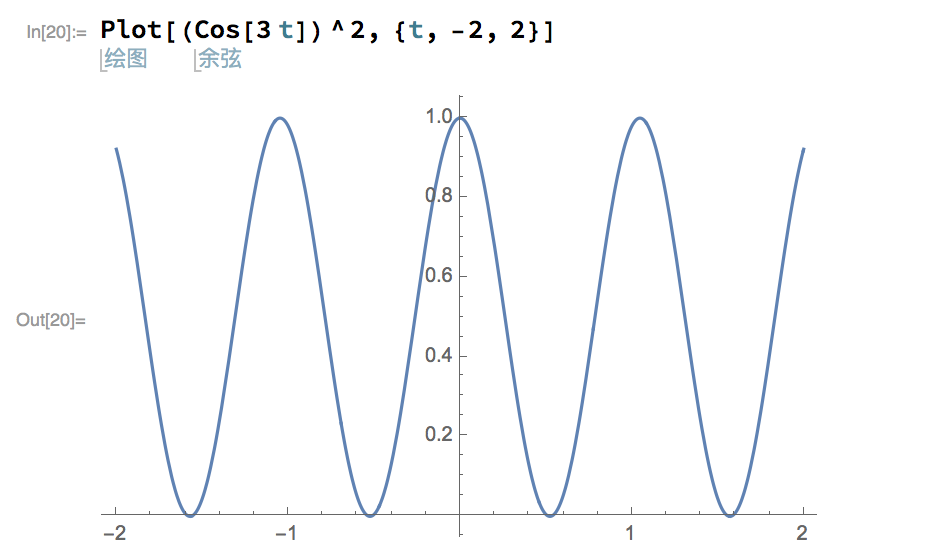
\includegraphics[width=8cm]{./Figures/20180305-cos3tsq.png}
  \label{fig:fourier-series-f-cos3tsq}
%
%  \small{Source: PBOC.}
\end{figure}

基准频率$\omega_{0} = \frac{2 \pi}{T} = 6$。已知
\begin{equation}
  \label{eq:fourier-series-expo-coef}
\begin{split}
  & \cos \left( 3t \right) = \frac{1}{2} \left[
  \exp \left( 3 i t \right) + \exp \left( - 3 i t \right)
  \right], \\
  & \hookrightarrow
  f(t) = \cos^{2} (3t) = \frac{1}{4} \left[
  \exp \left( 6 i t \right) + 2 + \exp \left( - 6 i t \right)
  \right], \\
  & \hookrightarrow
  \tilde{f}_{\nu} = \frac{1}{4 T} \int_{0}^{T}
  \exp \left( -i \nu \omega_{0} t \right)
  \left[
  \exp \left( i \omega_{0} t \right) + 2
  + \exp \left( - i \omega_{0} t \right)
  \right] \, \mathrm{d} t.
\end{split}
\end{equation}

根据正交性质(第\ref{eq:fourier-tips-orthogonal}节)可得,上式变为
\begin{equation*}
  \tilde{f}_{\nu} = \frac{1}{4}
  \left[
  \delta_{\nu,1} + 2 \delta_{\nu,0} + \delta_{\nu,-1}
  \right],
\end{equation*}
换句话说,傅里叶级数的系数$\tilde{f}_{\nu}$只有在$\nu = \left\{ -1, 0 ,1 \right\}$时不等于$0$。那么,将$f(t)$用傅里叶综合形式(第\ref{eq:fourier-series-synthesis}节)写为
\begin{equation}
  \label{eq:fourier-series-expo-coef-cal}
  \begin{split}
    f(t) & = \sum_{\nu} \tilde{f}_{\nu} \exp \left( - i \nu \omega_{0} t \right) = \frac{1}{4} \exp \left(i \omega_{0} t \right) + \frac{1}{2} + \frac{1}{4} \exp \left( - i \omega_{0} t \right) \\
    & = \frac{1}{2} \left[ 1 + \cos \left( \omega_{0} t \right) \right] = \frac{1}{2} \left[ 1 + \cos \left( 6 t \right) \right],
  \end{split}
\end{equation}

结合三角函数关系,上式还可以做进一步简化
\begin{equation*}
  \cos^{2} \left(3 t \right) = \frac{\cos \left( 6 t \right) + 1}{2}.
\end{equation*}

\subsubsection{傅里叶余弦级数}
\label{sec:fourier-series-sin-coef}

\eqref{eq:fourier-series-expo-coef-cal}将$f(t) = \cos^{2} \left( 3t \right)$分解为一个余弦项和一个常数项之和,没有正弦项。事实上若方程$f(t)$是偶函数,傅里叶变换后常常是没有正弦项的。反之亦然。我们将两种情况分别称为傅里叶余弦级数(Fourier cosine series)\index{Fourier cosine series \dotfill 傅里叶余弦级数}和傅里叶正弦级数(Fourier sine series)\index{Fourier sine series \dotfill 傅里叶正弦级数}。

有时候原始方程本身既不是奇函数也不是偶函数,但有可能通过坐标点的移动来变成奇或偶函数。如$T$-周期方程
\begin{equation*}
  f(t) = \begin{cases}
  0, & 0 < t < \frac{T}{2}\\
  1, & \frac{T}{2} < t < T
  \end{cases}
\end{equation*}
非奇非偶。可以设一个新函数$g(t) \equiv f \left( t + \frac{\pi}{4} \right)$,使得$g(t)$变成偶函数。

更一般地说,所有方程都可以分解为奇函数、偶函数组合的形式,如
\begin{equation*}
  \begin{split}
    f(t) & = f_{\text{偶}}(t) + f_{\text{奇}}(t), \\
    f_{\text{偶}}(t) & \equiv \frac{1}{2} \left[ f(t) + f(-t) \right], \\
    f_{\text{奇}}(t) & \equiv \frac{1}{2} \left[ f(t) - f(-t) \right].
  \end{split}
\end{equation*}

举例来说如锯齿波(sawtooth wave),$T$-周期方程$f(t)$在每一个周期内都满足$f(t) = t, \quad 0 < t < T$,也即,$f(t)$的单位与$t$的单位相同,都是时间,见图\ref{fig:fourier-series-sawwave}。
\begin{figure}[htbp]
   \caption{锯齿波}
  \centering
  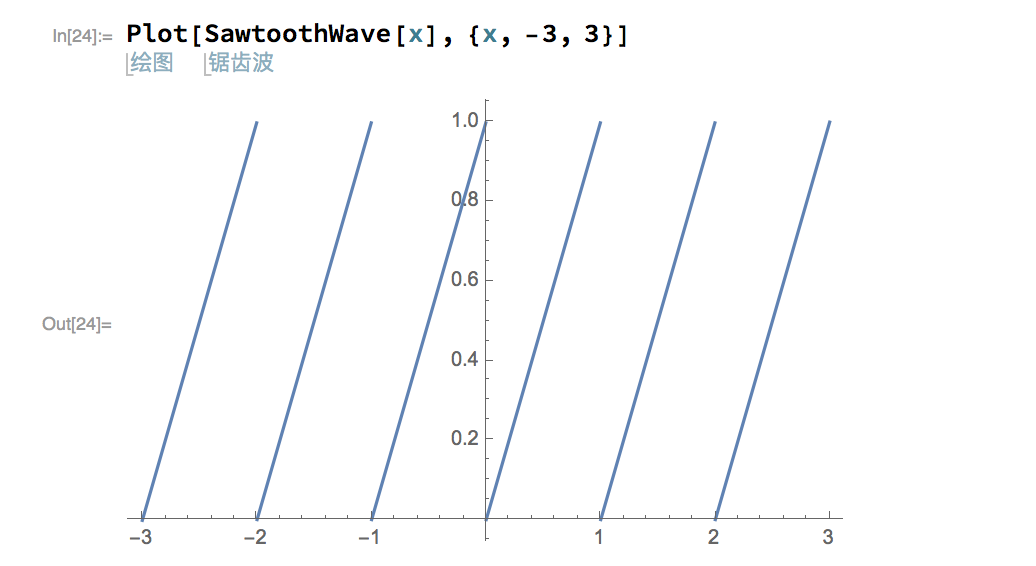
\includegraphics[width=8cm]{./Figures/20180305-sawtooth-wave.png}
  \label{fig:fourier-series-sawwave}
%
%  \small{Source: PBOC.}
\end{figure}

该方程的傅里叶级数
\begin{equation*}
  \begin{split}
    f(t) & = \sum_{\nu = - \infty}^{\infty} \tilde{f}_{\nu} \cdot \exp \left( i \nu \omega_{0} t \right), \quad \omega_{0} = \frac{2 \pi}{T}, \\
    \hookrightarrow \tilde{f}_{\nu} & = \frac{1}{T} \int_{0}^{T} f(t) \exp \left( - i \nu \omega_{0} t \right) \, \mathrm{d} t = \frac{1}{T} \int_{0}^{T} t \exp \left( - i \nu \omega_{0} t  \right) \, \mathrm{d} t.
  \end{split}
\end{equation*}

上式中$\tilde{f}_{\nu}$的值随着$\nu$的取值而不同,具体说来:
\begin{equation*}
  \tilde{f}_{0} = \frac{T}{2}, \quad \nu = 0,
\end{equation*}
\begin{equation*}
  \begin{split}
    \tilde{f}_{\nu} & = \frac{1}{T}
    \left[
    - \frac{1}{ i \nu \omega_{0}}
    \left| t \exp \left( - i \nu \omega_{0} t \right) \right|_{0}^{T}
    + \frac{1}{ i \nu \omega_{0}}
    \int_{0}^{T} \exp \left( - i \nu \omega_{0} t \right) \, \mathrm{d} t
    \right]  = - \frac{1}{i \nu \omega_{0}}, \quad \nu \neq 0.
  \end{split}
\end{equation*}

代回可得
\begin{equation*}
    \underbrace{
    \tilde{f}_{\nu}
    }_{\text{(时间)}} =
    \underbrace{
    \frac{T}{2}
    }_{\text{时间}}
     - \underbrace{
     \frac{1}{i \omega_{0}} \sum_{\nu = - \infty}^{\infty} \frac{1}{\nu} \exp \left( i \omega_{0} t \right)
     }_{\text{单位:(1/角频率)=时间}},
\end{equation*}
不难看出,在角频率$\omega$的值较大时,$\tilde{f}_{\nu}$以等比于$\frac{1}{\left| \omega \right|}$的速度衰减。这是由$f(t)$方程的非连续性所决定的(佩利——维纳诸定理, Theorem \ref{theorem:paley-wiener-theorems})。

上式也可改为正弦余弦形式
\begin{equation}
  \label{eq:fourier-series-sin-coef-sincos}
  f(t) = \frac{T}{2} - \underbrace{
  \frac{T}{\pi} \sum_{\nu = 1}^{\infty} \frac{1}{\nu}
  \sin \left(
  \frac{2 \nu \pi t}{T}
  \right)
  }_{\eqqcolon \mathcal{A}},
\end{equation}
其中$\mathcal{A}$符合傅里叶级数的特征。若设$g(t) = f(t) - \frac{T}{2}$,则$g(t)$就是个傅里叶正弦级数了——只要$g(t)$是一个奇函数的话——将图\ref{fig:fourier-series-sawwave}垂直下移$\frac{\pi}{2}$个单位不难看出,$g(t)$也是个奇函数。

\subsubsection{吉布斯现象}
\label{sec:fourier-series-gibbs-phenomenon}
前文可见,通过加总一系列弦波方程(假定其中每一个弦波都是平滑的),可以生成图\ref{fig:fourier-series-sawwave}一般参差状不连续的锯齿方程,但这是有限定条件的:如果我们只截取全部傅里叶级数中的一段,即只加总有限个项(总共有无数个项加总)的话,这意味着只对$f(t)$作有限个傅里叶综合的话,就会产生吉布斯现象(Gibbs phenomenon)\index{Gibbs phenomenon \dotfill 吉布斯现象}:这是指,在对非连续方程作不完全傅里叶综合时,在不连续点附近所出现的震荡。如图\ref{fig:fourier-series-gibbs-phenomenon}所示,原方程$f(t)$为锯齿方程,$f_{N}(t), n=2,5,10,20$分别为对$f(t)$所做的不完全傅里叶综合
\begin{equation*}
  f_{N}(t) = \sum_{\nu = - N}^{N} \tilde{f}_{\nu} \cdot \exp \left( i \nu \omega_{0} t \right).
\end{equation*}
不难看出,在远离不连续点(如$t=0,1$)的地方,$N$越是大,傅里叶级数越能对原方程作精确近似。而反之则不然:在接近不连续点的地方,傅里叶级数的近似精度并为随着$N$的升高而显著提升。

\begin{figure}[htbp]
   \caption{吉布斯现象}
  \centering
  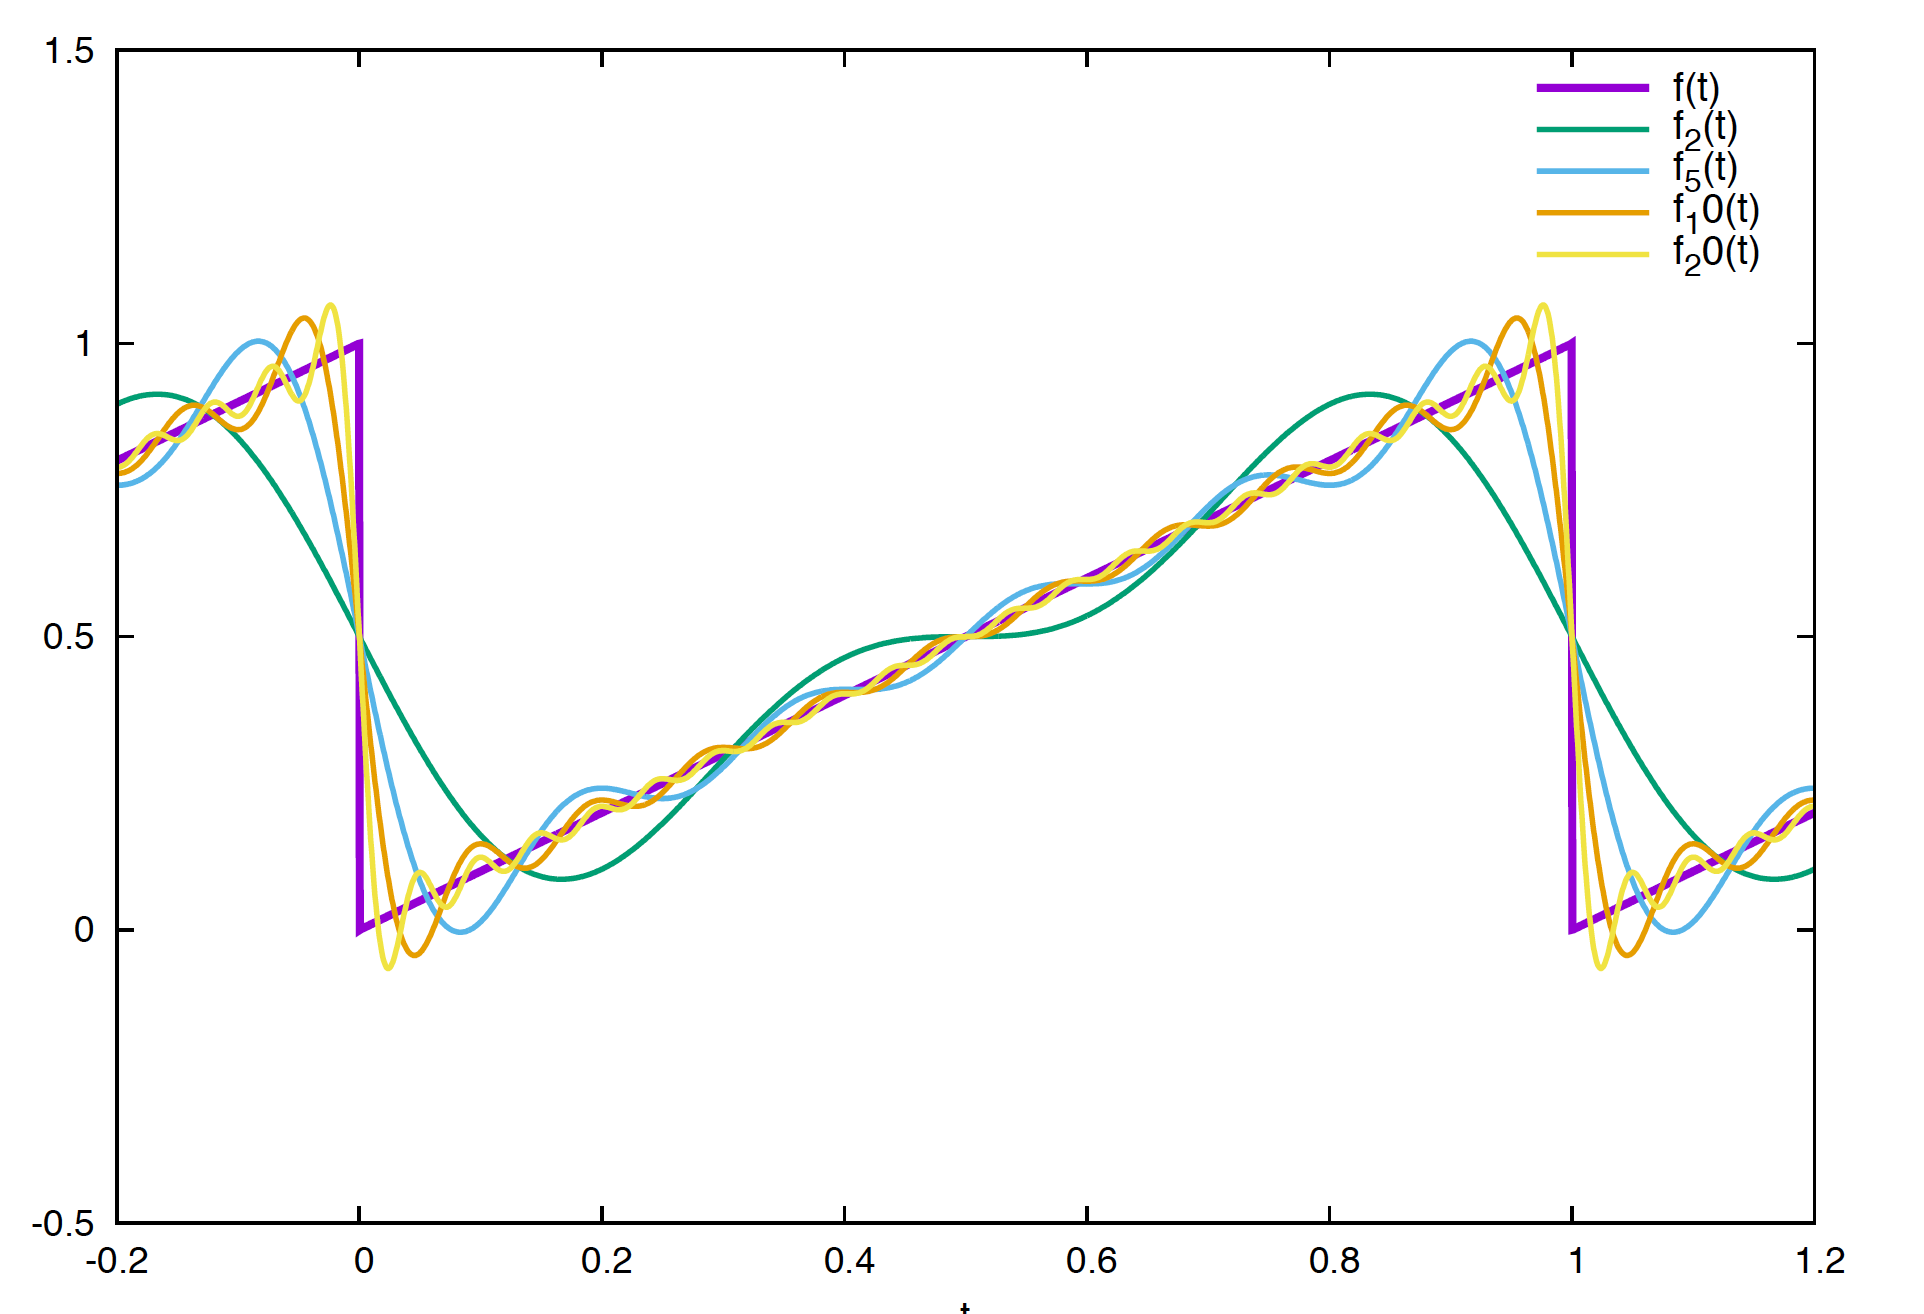
\includegraphics[width=10cm]{./Figures/20180305-gibbs-phenomenon.png}
  \label{fig:fourier-series-gibbs-phenomenon}
%
%  \small{Source: PBOC.}
\end{figure}

\subsubsection{傅里叶级数的收敛}
\label{sec:fourier-series-convergence}

图\ref{fig:fourier-series-gibbs-phenomenon}也揭示了傅里叶级数的又一个重要特征:如果非连续方程$f(t)$在$t^{*}$点不连续,那么它的傅里叶级数$\sum \tilde{f}_{\nu} \exp \left( i \nu \omega_{0} t^{*} \right)$收敛至这一不连续的中点,即
\begin{equation*}
\begin{split}
  & \lim_{N \rightarrow \infty}
  \sum_{\nu = - N}^{N}
  \tilde{f}_{\nu} \cdot \exp \left( i \nu \omega_{0} t^{*} \right)
  \approx \frac{1}{2}
  \left[
  f \left( t_{-}^{*}\right) + f \left( t_{+}^{*}\right)
  \right], \\
  & f \left( t_{-}^{*}\right) \equiv \lim_{\varepsilon \rightarrow 0} f \left( t^{*} - \varepsilon \right), \quad f \left( t_{+}^{*}\right) \equiv \lim_{\varepsilon \rightarrow 0} f \left( t^{*} + \varepsilon \right), \, \varepsilon > 0.
\end{split}
\end{equation*}

根据这一性质,如果我们在$[0,T]$区间内,对一个并非以$[0,T]$为周期的不连续方程作傅里叶级数的近似,那么用$t=0$点作傅里叶近似,可得$\frac{1}{2} \left[ f(0) + f(T)\right]$,这在图\ref{fig:fourier-series-gibbs-phenomenon}中有所反映。


\subsubsection{傅里叶分析是无损转换过程}
\label{sec:fourier-lossless}
傅里叶分析的又一个重要特征表现为,对原方程的傅里叶转换是无损(lossless)的,即$f(t)$中的信息在$f(t) \rightarrow \tilde{f}(\omega)$的过程中没有损耗。为了说明这一点,首先来介绍傅里叶综合(Fourier synthesis)\index{Fourier synthesis \dotfill 傅里叶综合}的概念:存在关于$f(t)$的傅里叶级数$\tilde{f}(\omega)$,并且可以根据傅里叶级数向回逆推得到原方程$f(t)$,表示为
\begin{equation}
  \label{eq:fourier-series-synthesis}
  f(t) = \int_{-\infty}^{\infty} \exp \left( i \omega t \right) \cdot \tilde{f}(\omega) \, \mathrm{d} \omega,
\end{equation}
即将一系列指数方程(或弦波曲线)加权加总,权重由与频率$\omega$有关的傅里叶变换$\tilde{f}(\omega)$给出;加总后的方程即原方程$f(t)$。

\begin{theorem}[帕赛瓦尔定理(傅里叶变换)]
\label{theorem:fourier-parseval-theorem}
我们说\eqref{eq:fourier-series-synthesis}是精确无损的,是指原域中的$f(t)$和傅里叶域中的$\tilde{f}(\omega)$之间相互转换不会产生信息损耗,这称为帕塞瓦尔定理(Parseval's theorem)。
\end{theorem}
\begin{proof}
  设两方程的内积(inner product)满足
  \begin{equation*}
    \langle f, g \rangle = \int_{-\infty}^{\infty} f^{*}(t) g(t) \, \mathrm{d}(t),
  \end{equation*}
  引入傅里叶综合形式\eqref{eq:fourier-series-synthesis}分别替代RHS被积方程中的$f^{*}$和$g(t)$,有
  \begin{equation}
    \label{eq:fourier-series-parseval-theorem}
    \begin{split}
      \langle f, g \rangle & = \int_{-\infty}^{\infty} f^{*}(t) g(t) \, \mathrm{d}(t) \\
      & = \int_{-\infty}^{\infty}
      \left\{
      \int_{- \infty}^{\infty}
      \exp \left( - i \omega t \right) \tilde{f}^{*} \left( \omega \right) \, \mathrm{d} \omega
      \right\}
      \cdot
      \left\{
      \int_{-\infty}^{\infty}
      \exp \left( i \omega^{'} t \right) \tilde{g} \left( \omega^{'} \right) \, \mathrm{d}\omega^{'}
      \right\}
      \, \mathrm{d} t \\
      & = \int_{-\infty}^{\infty}
      \tilde{f}^{*} \left( \omega \right)
      \int_{-\infty}^{\infty}
      \tilde{g} \left( \omega^{'} \right)
      \underbrace{
      \left\{
      \int_{-\infty}^{\infty}
      \exp \left[ i \left( \omega^{'} - \omega \right) t \right] \, \mathrm{d} t
      \right\}
      }_{= 2 \pi \delta \left( \omega^{'} - \omega \right)}
      \, \mathrm{d} \omega^{'} \, \mathrm{d} \omega \\
      & =
      \int_{-\infty}^{\infty}
      \tilde{f}^{*} \left( \omega \right)
      \int_{-\infty}^{\infty}
      \tilde{g} \left( \omega^{'} \right)
      2 \pi \delta \left( \omega^{'} - \omega \right)
      \, \mathrm{d} \omega^{'} \, \mathrm{d} \omega \\
      & = 2 \pi \int_{-\infty}^{\infty}
      \tilde{f}^{*} \left( \omega \right)
      \tilde{g} \left( \omega \right)
      \, \mathrm{d} \omega,
    \end{split}
  \end{equation}
  也就是说,原方程的内积$\langle f,g \rangle$等于它们两个的傅里叶变换相乘$\tilde{f}^{*}\left( \omega \right) \tilde{g} \left( \omega \right)$后的积。
\end{proof}

\begin{theorem}[普朗歇尔定理(傅里叶变换)]
  \label{theorem:fourier-series-plancherel-theorem}
在帕塞瓦尔定理(Theorem \ref{theorem:fourier-parseval-theorem})的基础上,设$f(t) \equiv g(t)$,那么由式\eqref{eq:fourier-series-parseval-theorem}可得
\begin{equation}
  \label{eq:fourier-series-plancherel-theorem}
  \langle f, g \rangle = \int_{-\infty}^{\infty} \left| f(t) \right|^{2} \, \mathrm{d} t
  = 2 \pi \int_{-\infty}^{\infty} \left| \tilde{f} \left( \omega \right) \right|^{2} \, \mathrm{d} \omega,
\end{equation}
又称普朗歇尔定理(Plancherel's theorem)\index{Plancherel's theorem \dotfill 普朗歇尔定理}。
\end{theorem}

现在将区间$\left( - \infty, \infty \right)$缩小到某个定区间$\left[ 0, T \right]$,来看傅里叶级数中方程转换的信息损耗问题。之所以关注定区间$\left[ 0, T \right]$,要么是因为原方程$f(t)$是$T$-周期方程,要么是我们的研究中只关注特定区间内方程值的变化。
\begin{theorem}[帕赛瓦尔定理(傅里叶级数)]
\label{theorem:fourier-parseval-theorem-series}
在$[0,T]$区间内,由Theorem \ref{theorem:fourier-parseval-theorem}可得
\begin{equation}
  \label{eq:fourier-parseval-theorem-series}
  \int_{0}^{T} f^{*} \left( t \right) g \left( t \right) \, \mathrm{d} t
  = T \sum_{\nu = - \infty}^{\infty} \tilde{f}_{\nu}^{*} \tilde{g}_{\nu}.
\end{equation}
\end{theorem}

\begin{theorem}[普朗歇尔定理(傅里叶级数)]
  \label{theorem:fourier-series-plancherel-theorem-series}
在$[0,T]$区间内,由Theorem \ref{theorem:fourier-series-plancherel-theorem}可得
\begin{equation}
  \label{eq:fourier-series-plancherel-theorem-series}
  \int_{0}^{T} \left| f(t) \right|^{2} \, \mathrm{d} t
  = T \sum_{\nu = - \infty}^{\infty} \left| \tilde{f}_{\nu} \right|^{2}.
\end{equation}
\end{theorem}

根据帕塞瓦尔定理和普朗歇尔定理,在数值计算过程中,我们既可以求解实区间中的原始方程,也可以求解傅里叶空间中的变换方程,二者等价。实际求解哪一种取决于哪个更容易计算。

\subsection{泊松求和式}
\label{sec:fourier-poisson-summation-formula}
采用类似于帕塞瓦尔定理的思路,也有另一种在实域或傅里叶域近似求积的方法,称泊松求和式(Poisson summation formula)\index{Poisson summation formula \dotfill 泊松求和式}。
\begin{theorem}
  具体说来,假定关于方程$f(t)$,我们想要求得一组等宽分布的时间点(对应宽度$\Delta t$)下$f(t)$值的和。根据泊松求和式,我们也可以计算傅里叶域中一组等宽分布(对应宽度$\frac{2 \pi}{\Delta t}$)的$\tilde{f}\left( \omega \right)$的值,两种方法等价。

  \begin{equation}
    \label{eq:fourier-poisson-summation-formula}
    \sum_{n = - \infty}^{\infty} f \left( n \Delta t \right)
    =
    \frac{2 \pi}{\Delta t}  \sum_{\nu = - \infty}^{\infty}
    \tilde{f} \left( \frac{2 \pi \nu}{\Delta t} \right).
  \end{equation}
\end{theorem}
\begin{proof}
  用傅里叶综合表达式改写\eqref{eq:fourier-poisson-summation-formula}LHS
  \begin{equation*}
    \begin{split}
      \sum_{n=-\infty}^{\infty} f \left( n \Delta t \right)
      & =
      \sum_{n=-\infty}^{\infty}
      \left[
      \int_{-\infty}^{\infty} \tilde{f} \left( \omega \right)
      \exp \left( i n \omega \Delta t \right) \, \mathrm{d} \omega
      \right]\\
      & = \int_{-\infty}^{\infty} \tilde{f} \left( \omega \right)
      \underbrace{
      \sum_{n=-\infty}^{\infty}
      \exp \left( i n \omega \Delta t \right)
      }_{= 2 \pi \sum_{\nu} \delta \left( \omega \Delta t - 2 \nu \pi \right)}
      \, \mathrm{d} \omega \\
      & = \int_{-\infty}^{\infty} \tilde{f} \left( \omega \right)
      2 \pi \underbrace{
      \sum_{\nu} \delta \left( \omega \Delta t - 2 \nu \pi \right)
      }_{\eqqcolon \mathcal{A}}
      \, \mathrm{d} \omega,
    \end{split}
  \end{equation*}

  最后一行等式中,将$f \left( n \Delta t \right)$理解为一个关于$\omega \Delta t - 2 \nu \pi$的狄拉克方程,可分两种情况进一步分析
  \begin{itemize}
    \item 如果$\omega \Delta t$是$2 \pi$的整数倍($\nu \in \mathcal{Z}$可以是任意整数),那么$\sum_{n=-\infty}^{\infty} f \left( n \Delta t \right) = \infty$。
    \item 否则,$\mathcal{A}$就是一组狄拉克方程$\delta \left( \omega \Delta t - 2 \nu \pi \right)$之和,每个狄拉克方程对应不同的$\nu$值;进而
    $\sum_{n=-\infty}^{\infty} f \left( n \Delta t \right) =0$,各项之间相互抵消。
  \end{itemize}

由狄拉克方程的性质
\begin{equation*}
  \delta \left( a x - b \right) = \frac{1}{a} \delta \left( x - \frac{b}{a} \right)
\end{equation*}
可进一步得到

\begin{equation*}
\begin{split}
    \sum_{n=-\infty}^{\infty} f \left( n \Delta t \right)
    & = 2 \pi \sum_{\nu} \int_{-\infty}^{\infty} \tilde{f} \left( \omega \right) \delta \left( \omega \Delta t - 2 \nu \pi \right) \, \mathrm{d} \omega\\
    & = \frac{2 \pi}{\Delta t} \sum_{\nu} \int_{-\infty}^{\infty}
    \tilde{f} \left( \omega \right)
    \delta \left( \omega - \frac{2 \nu \pi}{\Delta t} \right) \, \mathrm{d} \omega\\
    & = \frac{2 \pi}{\Delta t} \sum_{\nu = - \infty}^{\infty} \tilde{f} \left( \nu \frac{2 \pi}{\Delta t} \right),
\end{split}
\end{equation*}
证毕。
\end{proof}

两个值域中各有一组点,两组点的单位相同\footnote{
$\tilde{f}$的单位=$f$的单位/频率=$f$的单位$\times$(时间),其中时间用$\Delta t$来表示。因此$\tilde{f}$的单位/$\Delta t$=$f$的单位。}。
为了简化表达,设$\Delta \omega \equiv \frac{2 \pi}{\Delta t}$,则\eqref{eq:fourier-poisson-summation-formula}改写为
\begin{equation}
  \label{eq:fourier-poisson-summation-formula-simp}
  \sum_{n = - \infty}^{\infty} f \left( n \Delta t \right)
  = \Delta \omega \sum_{\nu = - \infty}^{\infty}
  \tilde{f} \left( \nu \cdot \Delta \omega \right),
\end{equation}
值得留意的是$\Delta t$和$\Delta \omega$呈反比例,即,在原时间域中,若是对原方程$f(t)$取密集的配点求$\sum f(\cdot)$,对应较小的$\Delta t$值,那么在对应的傅里叶域中,就涉及到较高的频率值$\Delta \omega$——换句话说,原域中的配点越是密,在稀疏频率域中对应的点就越是稀疏。

随着$f(\cdot)$的形式不同,泊松求和式的一些具体应用如下。

\subsubsection{高斯方程的泊松求和}
\label{eq:fourier-poisson-gaussian}

在前面介绍过,一个高斯方程的傅里叶变换也是一个高斯方程(第\ref{sec:fourier-gaussian}节)。结合本节的知识我们可以作进一步判断:对高斯方程形式原方程配点越宽(如,实域宽度$\sigma$),其变换后的高斯形式方程越窄(如,傅里叶域对应的宽度$\frac{2}{\sigma}$)。

因此,设一个以$x$为参数的关于$t$的高斯方程$ T_{x}(t)=\exp \left( - t^{2} \pi x \right)$,要求$\sum T_{x}(t)$。在$\sum T_{x}(t)$的收敛速度较慢的情况下,我们可以利用泊松求和式,在傅里叶空间中进行求和计算\footnote{快速收敛的原因可能如,$\pi x$的值较小,从而导致$\sum T_{x}(t)$收敛缓慢。}。具体说来,$T_{x}(t)$的傅里叶变换
\begin{equation*}
  \begin{split}
    \widetilde{T}_{x} \left( \omega \right)
    & = \frac{1}{2 \pi} \int_{-\infty}^{\infty} \exp \left( - i \omega t \right) T_{x}(t) \, \mathrm{d} t \\
    & = \frac{1}{2 \pi} \int_{-\infty}^{\infty}
    \exp \left( - i \omega t - t^{2} \pi x \right)  \, \mathrm{d} t \\
    & = \frac{1}{2 \pi \sqrt{x}}
    \exp \left(
    - \frac{\omega^{2}}{4 \pi x}
    \right),
  \end{split}
\end{equation*}

\subsubsection{雅各比方程}
\label{sec:fourier-poisson-jacobian}
雅各比方程族(Jacobian $\theta$ function)\index{Jacobian function \dotfill 雅各比方程}中的一种形式可以表示为
\begin{equation}
  \label{eq:fourier-poisson-jacobian}
  \theta(x) = \sum_{n = - \infty}^{\infty}
  \exp \left( - n^{2} \pi x \right)
  = \sum_{n = - \infty}^{\infty} T_{x}(n).
\end{equation}

利用泊松求和式\eqref{eq:fourier-poisson-summation-formula},以及设$\Delta t = 1$,有
\begin{equation}
\label{eq:fourier-poisson-jacobian-2}
\theta(x) = 2 \pi \sum_{\nu = - \infty}^{\infty} \widetilde{T} \left( 2 \nu \pi \right)
= \frac{1}{\sqrt{x}}
\underbrace{
\sum_{\nu = - \infty}^{\infty}
\exp \left(
 - \frac{\pi \nu^{2}}{x}
\right)
}_{= \theta \left( \frac{1}{x} \right)},
\end{equation}

即雅各比方程\eqref{eq:fourier-poisson-jacobian}的函数方程(functional equation)形式
\begin{equation}
\label{eq:fourier-poisson-jacobian-equiv}
\begin{split}
  \theta \left( x \right) & = \frac{1}{\sqrt{x}} \theta \left( \frac{1}{x} \right),\\
  \Leftrightarrow \sum_{n = - \infty}^{\infty}
  \exp \left( - n^{2} \pi x \right) & = x^{-\frac{1}{2}} \sum_{\nu = - \infty}^{\infty} \exp \left( - \frac{\nu^{2} \pi }{x} \right).
\end{split}
\end{equation}

% Table generated by Excel2LaTeX from sheet 'Sheet1'
\begin{table}[htbp]
\centering
\caption{雅各比方程的泊松求和}
  \begin{tabular}{|l|r|rrr}
  \toprule
        & \multicolumn{2}{c|}{LHS} & \multicolumn{2}{c|}{RHS} \\
  \midrule
  $n(\nu)$ & \multicolumn{1}{l|}{$\exp \left( -n^{2} \pi x \right)$} & \multicolumn{1}{l|}{$\sum_{n} \exp \left( -n^{2} \pi x \right)$} & \multicolumn{1}{l|}{$\exp \left( -\nu^{2} \pi / x \right)$} &
  \multicolumn{1}{l|}{$\sum_{\nu} \exp \left( -\nu^{2} \pi / x \right)$} \\
  \midrule
  \multicolumn{1}{|r|}{0} & 1.000000000 & \multicolumn{1}{r|}{1.000000000} & \multicolumn{1}{r|}{1.000000000} & \multicolumn{1}{r|}{5.000000000} \\
  \midrule
  \multicolumn{1}{|r|}{1} & 0.881911378 & \multicolumn{1}{r|}{2.763822757} & \multicolumn{1}{r|}{7.77304E-35} & \multicolumn{1}{r|}{5.000000000} \\
  \midrule
  \multicolumn{1}{|r|}{2} & 0.604922563 & \multicolumn{1}{r|}{3.973667882} & \multicolumn{1}{r|}{3.6506E-137} & \multicolumn{1}{r|}{5.000000000} \\
  \midrule
  \multicolumn{1}{|r|}{3} & 0.322718983 & \multicolumn{1}{r|}{4.619105849} & \multicolumn{1}{r|}{1.0359E-307} & \multicolumn{1}{r|}{5.000000000} \\
  \midrule
  \multicolumn{1}{|r|}{4} & 0.133905721 & \multicolumn{1}{r|}{4.886917291} & \multicolumn{1}{r|}{0} & \multicolumn{1}{r|}{5.000000000} \\
  \midrule
  \multicolumn{1}{|r|}{5} & 0.043213918 & \multicolumn{1}{r|}{4.973345128} & \multicolumn{1}{r|}{0} & \multicolumn{1}{r|}{5.000000000} \\
  \midrule
  \multicolumn{1}{|r|}{6} & 0.010846711 & \multicolumn{1}{r|}{4.995038549} & \multicolumn{1}{r|}{0} & \multicolumn{1}{r|}{5.000000000} \\
  \midrule
  \multicolumn{1}{|r|}{7} & 0.002117495 & \multicolumn{1}{r|}{4.999273539} & \multicolumn{1}{r|}{0} & \multicolumn{1}{r|}{5.000000000} \\
  \midrule
  \multicolumn{1}{|r|}{8} & 0.000321512 & \multicolumn{1}{r|}{4.999916562} & \multicolumn{1}{r|}{0} & \multicolumn{1}{r|}{5.000000000} \\
  \midrule
  \multicolumn{1}{|r|}{9} & 3.79683E-05 & \multicolumn{1}{r|}{4.999992498} & \multicolumn{1}{r|}{0} & \multicolumn{1}{r|}{5.000000000} \\
  \midrule
  \multicolumn{1}{|r|}{10} & 3.48734E-06 & \multicolumn{1}{r|}{4.999999473} & \multicolumn{1}{r|}{0} & \multicolumn{1}{r|}{5.000000000} \\
  \midrule
  \multicolumn{1}{|r|}{11} & 2.49126E-07 & \multicolumn{1}{r|}{4.999999971} & \multicolumn{1}{r|}{0} & \multicolumn{1}{r|}{5.000000000} \\
  \midrule
  x=    & 0.04  &       &       &  \\
\cmidrule{1-2}    \end{tabular}%
\label{tab:fourier-poisson-jacobian-equiv}%

\small{注:基于式\eqref{eq:fourier-poisson-jacobian-equiv}计算。excel表格见文件夹中data/20180306-poisson.xlsx .}
\end{table}%

为了说明为何傅里叶级数求和的形式即\eqref{eq:fourier-poisson-jacobian-equiv}RHS更适于进行数值计算,我们做了一个小实验,设$x=0.04$,$n=0,1,\ldots,11$。不难看出,LHS需要$n=11$,前后23项的求和才能达到小数点后6位的精度;而对于雅各比方程形式的傅里叶级数求和,RHS只需要$n=1$就能达到同样的精度,换句话说,由\eqref{eq:fourier-poisson-jacobian-equiv}我们有
\begin{equation*}
\underbrace{
\theta \left( 0.04 \right)
}_{4.999999971, n=11}
=
\underbrace{
\frac{1}{\sqrt{0.04}}
}_{5.0}
\underbrace{
\theta \left( \frac{1}{0.04} \right)
}_{1.000000000, \nu = 1}
\end{equation*}

\subsection{傅里叶分析与卷积}
\label{sec:fourier-series-convolution}
傅里叶分析的又一个重要特征是,它是以卷积(convolution)\index{convolution \dotfill 卷积}乘的形式出现的。如上文所示,由两个方程$f(t)$和$g(t)$构成的卷积,近似表示为一系列$g(\tau)$的加权和,$g(\tau)$是对$g(t)$的近似(copy)之一,对应权重$f(\tau)$,我们设这个卷积为$C(t)$
\begin{equation*}
C(t) \equiv f \times g = \int_{-\infty}^{\infty} f(\tau) g(t - \tau) d \tau.
\end{equation*}

对$C(t)$作傅里叶变换,有
\begin{equation*}
\begin{split}
\widetilde{C}(\omega) & = \frac{1}{2 \pi}
\int_{-\infty}^{\infty} C(t) \exp \left( - i \omega t \right) \, \mathrm{d} \omega  \\
& = \frac{1}{2 \pi} \int_{-\infty}^{\infty}
\int_{-\infty}^{\infty} f(\tau) g(t - \tau)
\, \mathrm{d} \omega
\exp \left( - i \omega t \right)
\, \mathrm{d} t.
\end{split}
\end{equation*}

将上式中的$f(\tau)$和$g(t - \tau)$替换为傅里叶综合形式
\begin{equation*}
\begin{split}
  \widetilde{C} \left( \omega \right) & =
  \frac{1}{2 \pi} \int_{-\infty}^{\infty}
  \int_{-\infty}^{\infty}
  \left\{
  \int_{-\infty}^{\infty}
  \exp \left( i \omega_{1} \tau \right)
  \tilde{f} \left( \omega_{1} \right)
  \, \mathrm{d} \omega_{1}
  \right\}
  \left\{
  \int_{-\infty}^{\infty}
  \exp \left[ i \omega_{2} \left( t - \tau \right)  \right]
  \tilde{g} \left( \omega_{2} \right)
  \, \mathrm{d} \omega_{2}
  \right\}
  \exp \left( - i \omega t \right)
  \, \mathrm{d} \tau
  \, \mathrm{d} t \\
  & = \frac{1}{2 \pi} \int_{-\infty}^{\infty}
  \int_{-\infty}^{\infty}
  \left\{
  \int_{-\infty}^{\infty}
  \exp \left[
  i \left( \omega_{1} - \omega_{2} \right) \tau
  \right]
  \, \mathrm{d} \tau
  \right\}
  \left\{
  \int_{-\infty}^{\infty}
  \exp \left[
  i \left( \omega_{2} - \omega_{2} \right) t
  \right]
  \, \mathrm{d} t
  \right\}
  \tilde{f} \left( \omega_{1} \right)
  \tilde{g} \left( \omega_{2} \right)
  \, \mathrm{d} \omega_{1}
  \, \mathrm{d} \omega_{2} \\
  & = \frac{1}{2 \pi} \int_{-\infty}^{\infty}
  \int_{-\infty}^{\infty}
  \left[ 2 \pi \delta \left( \omega_{1} - \omega_{2} \right) \right]
  \left[ 2 \pi \delta \left( \omega_{2} - \omega \right) \right]
  \tilde{f} \left( \omega_{1} \right)
  \tilde{g} \left( \omega_{2} \right)
  \, \mathrm{d} \omega_{1}
  \, \mathrm{d} \omega_{2} \\
  & = 2 \pi
  \tilde{f} \left( \omega \right)
  \tilde{g} \left( \omega \right),
\end{split}
\end{equation*}
上式告诉我们,$f$和$g$的卷积的频率为$\omega$的傅里叶变换系数$\widetilde{C}\left( \omega \right)$,就等于$f$和$g$分别的$\omega$频率傅里叶系数之积。这意味着在频率域中进行卷积运算,要比在原始实值域中做卷积运算更方便一些。

\subsection{高维傅里叶变换}
\label{eq:fourier-transform-higher}
更高维度傅里叶变换的方法,与一维傅里叶变换类似。例如对二维方程$f(x,y)$而言,第一步保持$x$不变,做关于$y$的傅里叶变换,可得一个混合了实空间和傅里叶空间的方程$\tilde{f} \left( x,k_{y} \right)$
\begin{equation*}
\tilde{f} \left( x , k_{y} \right) = \frac{1}{2 \pi}
\int_{\infty}^{\infty} \exp \left( - i k_{y} y \right) f \left( x,y \right) \, \mathrm{d} y.
\end{equation*}

第二步保持$k_{y}$不变,再对$\tilde{f} \left( x,k_{y} \right)$做关于$x$的傅里叶变换,得到$\tilde{f} \left( k_{x} ,k_{y} \right)$
\begin{equation*}
\begin{split}
  \widetilde{f} \left( k_{x}, k_{y} \right)
  & = \frac{1}{2 \pi} \int_{-\infty}^{\infty} \exp \left( - i k_{x} x \right) \tilde{f} \left( x , k_{y} \right) \, \mathrm{d} x \\
  & = \left( 2 \pi \right)^{-2}
  \int_{-\infty}^{\infty}
  \exp \left( - i k_{x} x \right)
  \int_{-\infty}^{\infty}
  \exp \left( - i k_{y} y \right)
  f \left( x, y \right)
  \, \mathrm{d} y
  \, \mathrm{d} x \\
  & = \left( 2 \pi \right)^{-2}
  \int_{-\infty}^{\infty}
  \int_{-\infty}^{\infty}
  \exp \left[ - i \left( k_{x} x + k_{y} y \right) \right]
  f \left( x, y \right)
  \, \mathrm{d} y
  \, \mathrm{d} x \\
  & = \left( 2 \pi \right)^{-2}
  \int \exp \left( - i \cdot \bm{k} \cdot \bm{x} \right)
  \mathrm{d} \bm{x},
\end{split}
\end{equation*}
其中积分符号表示解释变量$\bm{x}$的全部取值区间。

$D$维方程也可用类似地方式求得,前缀系数此时变为$\left( 2 \pi \right)^{- D}$。

\subsection{一些指数求和的背景知识}
\label{sec:fourier-expo-sums}

\subsubsection{连续、有限时间域}
假定一个连续、有限的时间区间,宽度为$T$,那么方程$f(t)$在傅里叶域中的基准频率为$\omega_{0} = \frac{2 \pi}{T}$。进而我们有
\begin{equation}
\label{eq:fourier-tips-continue}
\frac{1}{T} \int_{0}^{T} \exp \left( n_{1} - n_{2} \right) \omega_{0} t \, \mathrm{d} t = \delta \left(n_{1}, n_{2} \right),
\end{equation}
其中$\delta \left(n_{1}, n_{2} \right)$表示克罗内克乘积,见\eqref{eq:poly-kronecker}。

\subsubsection{正交性}
\label{eq:fourier-tips-orthogonal}
\eqref{eq:fourier-tips-continue}中,如果$n_{1} \neq n_{2}$,那么我们可以说,方程$f_{n_{1}}(t) = \exp \left( i n_{1} \omega_{0} t \right)$和$f_{n_{2}}(t) = \exp \left( i n_{2} \omega_{0} t \right)$在内积的意义上正交(orthogonal),可表示为
\begin{equation*}
\langle f, g \rangle = \frac{1}{T} \int f^{*} g \, \mathrm{d} t.
\end{equation*}

更多正交性条件的介绍,见第\ref{eq:poly-orthogonality-types}节。

\subsubsection{连续、无限时间域}
\label{eq:fourier-tips-cont-infty}

在连续、无限时间域中,\eqref{eq:fourier-tips-continue}就变成了
\begin{equation}
\label{eq:fourier-tips-continue-infty}
\int_{-\infty}^{\infty}
\left[
i \left( \omega - \omega^{'}  \right) t
\right] \, \mathrm{d} t = 2 \pi \delta \left( \omega - \omega^{'} \right).
\end{equation}

\subsubsection{离散时间域}
\label{eq:fourier-tips-discrete-infty}

上文在第\ref{sec:fourier-series-convolution}节做泊松求和时,用到了\eqref{eq:fourier-tips-continue-infty},以处理连续、无限时间域中的求积问题。对应的离散傅里叶变换版本可写作
\begin{equation*}
\sum_{n = - \infty}^{\infty} \exp \left( i n k x \right) = 2 \pi \sum_{\nu = - \infty}^{\infty} \delta \left( x k - 2 \nu \pi \right),
\end{equation*}
RHS中,如果$x$等于$\frac{2\pi}{k}$的整数倍,那么LHS是$\infty$:$\exp \left( i n k x \right) = 1 \, \forall n$,$\sum_{n} 1 = \infty$。如果不是整数倍,$LHS$的无数个$\exp \left( i n k x \right)$相互抵消,LHS $= 0$。

来看是整数倍,进而LHS$=\infty$时的情况。若将左侧进一步扩展为$\int f(x) \exp \left( i n k x \right) \, \mathrm{d} x$(对$x$求积分),那么我们将得到一个$ < \infty$的数值,数值的大小取决于$x = \frac{2 \nu \pi}{k}$时对应的$f(x)$的值。

\subsubsection{高斯求积}
\label{sec:fourier-tips-gaussian}
第\ref{sec:fourier-gaussian}节介绍高斯变换时,使用了一个较为复杂的高斯方程。高斯方程族中,一个基本的高斯求积问题可以表示为
\begin{equation}
\label{eq:fourier-tips-gaussian-basic}
\int_{\infty}^{\infty} \exp \left( - x^{2} \right) \, \mathrm{d} x
= \sqrt{\pi}.
\end{equation}

稍稍做个扩展,在指数项中放入一个系数$\alpha$,则\eqref{eq:fourier-tips-gaussian-basic}调整为
\begin{equation}
\label{eq:fourier-tips-gaussian-ext}
\int_{-\infty}^{\infty} \exp \left( - \alpha x^{2} \right) \, \mathrm{d} x = \sqrt{\frac{\pi}{\alpha}}.
\end{equation}

再继续做扩展,一个高斯求积
\begin{equation*}
I\left( \alpha, \beta, \gamma \right)
= \int_{-\infty}^{\infty} \exp \left( - \alpha x^{2} + \beta x + \gamma \right) \, \mathrm{d} x,
\end{equation*}
求解方法如下:
\begin{itemize}
\item 提取出常数项$\gamma$
\begin{equation*}
  \begin{split}
  I \left( \alpha, \beta, \gamma \right)
  & = \exp \left( \gamma \right)
  \int_{-\infty}^{\infty} \exp \left( \underbrace{
  - \alpha x^{2} + \beta x
  }_{
  = - \alpha \left( x - \frac{\beta}{2 \alpha} \right)^{2} + \frac{\beta^{2}}{4 \alpha}
  }
  \right) \, \mathrm{d} x \\
  & = \exp \left( \gamma + \frac{\beta^{2}}{4 \alpha} \right)
  \int_{-\infty}^{\infty}
  \exp \left(
  - \alpha \left[ x - \frac{\beta}{2 \alpha} \right)^{2}
  \right] \, \mathrm{d} x.
\end{split}
\end{equation*}
\item 设$y \equiv x - \frac{\beta}{2 \alpha}$。上式变为
\begin{equation*}
\begin{split}
  I \left( \alpha, \beta, \gamma \right)
  & = \exp \left( \gamma + \frac{\beta^{2}}{4 \alpha} \right)
  \underbrace{
  \int_{-\infty}^{\infty}
  \exp \left(
    - \alpha y^{2}
    \right) \, \mathrm{d} y
    }_{= \sqrt{\frac{\pi}{\alpha}}}\\
    & = \sqrt{\frac{\pi}{\alpha}} \exp \left( \gamma + \frac{\beta^{2}}{4 \alpha} \right).
\end{split}
\end{equation*}
\end{itemize}










\end{subappendices}
